\documentclass{udpreport}
\title{Topología Física y Lógica de una red LAN}
\author{Integrantes: Thomas Muñoz, Ignacio Yanjari, Dagoberto Navarrete, Ignacio López.}
\date{Marzo de 2016}
\usepackage{graphicx}
\graphicspath{ {img/} }
\udpschool{Escuela de Informática y Telecomunicaciones}

\begin{document}
\maketitle
\tableofcontents
\chapter{Introducción}
	        En este laboratorio se buscó reconocer y comprender la composición de la red del laboratorio de Informática, 
	        identificando el hardware de red y los elementos que forman parte de este, ya sean computadores, cables, dispositivos 
	        de red (tales como el servidor, el router y el switch), etc. También se realizó un diagrama de red, el cual especifica
	        la información de los dispositivos que conforman la red, como sus IP's o MAC's y la topología que se está utilizando.
\chapter{Actividades}
	\section{Identificación de elementos de red}
		"Lo primero que se procede a identificar es el computador, ya que este es el que teníamos más cercano, para eso vimos 		el costado izquierdo de la CPU el cual tenía el número de serie del computador y el modelo. Después se procedió a identifiacr 		el cable de conexión a red ya que este era solo mirar la parte trasera del computador y ahí se encontraba, al ver el cable 		a lo largo se identifica que es un cable Fastlink categoría 5e UTP. Después se identifica el switch y el patch panel, los 		cuales se encontraban en la esquina superior derecha del laboratorio, en estos equipos estaba impresa su marca y modelo 		los cuales eran cisco series 2960 y Siemon hd-5e respectivamente. Finalmente se procede a identificar cada equipo en 			el switch para lo cual se tuvo que ir desconectando equipo por equipo y verificar la luz que se apagaba, esa era el 		número que identificaba en el switch, después se desconectó cada equipo para ver su equivalencia en el patch panel.\\
		A continuación se mostraran las características y especificaciones técnicas de los equipos mencionados en el párrafo 			anterior\\
\begin{itemize}
		\item{\bf-Tipo:} Computador de escritorio\\
		\item{\bf-Modelo:}  HP EliteDesk 800 G1 con factor de forma reducido (ENERGY STAR)
		(K6P73LT)\\
		\begin{figure}[h]
    		\centering
    	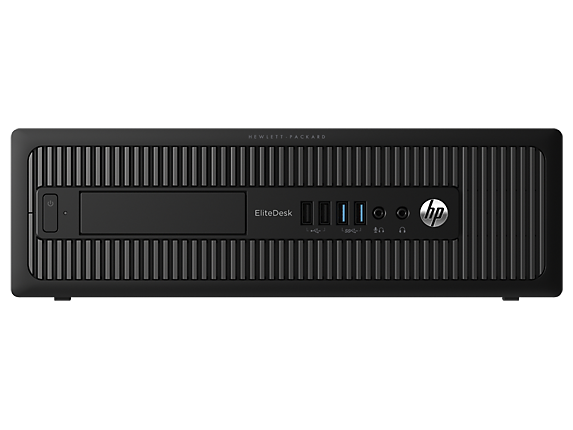
\includegraphics[width=\textwidth]{pchp1.png}
		\end{figure}
		\begin{figure}[h]
    		\centering
    	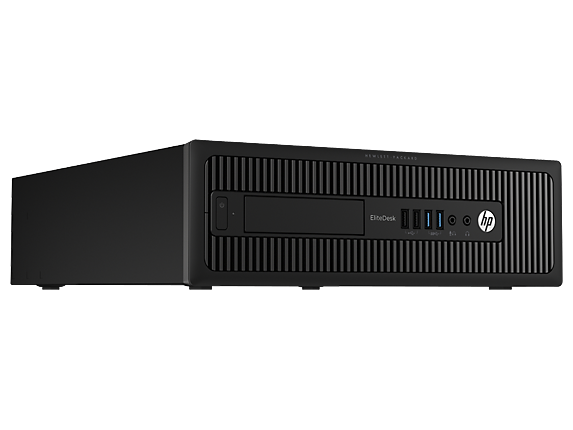
\includegraphics[width=\textwidth]{pchp2.png}
		\end{figure}
		\item{\bf-Especificaciones:}
		\begin{itemize}
			\item Procesador:Intel® Core™ i7-4790 con gráficos Intel HD 4600 (3,6 GHz, 8 MB de caché, 4 núcleos)\\
			\item Memoria, estándar:SDRAM DDR3 de 8 GB y 1600 MHz (1 x 8 GB)\\
			\item Unidad interna:SATA de 1 TB y 7200 rpm\\
			\item Unidad óptica:Grabadora SATA de DVD SuperMulti delgada\\
			\item Gráficos:Gráficos Intel HD 4600\\
			\item Interfaz de red:Conexión de red Intel I217LM GbE integrada\\
		\end{itemize}
		\item{\bf-Tipo:} Switch\\
		\item{\bf-Modelo:} Cisco Catalyst 2960-24TT-L Switch\\
		\begin{figure}[h]
    		\centering
    	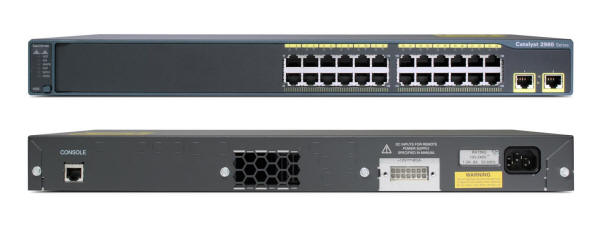
\includegraphics[width=\textwidth]{switch.jpg}
		\end{figure}
		\item{\bf-Especificaciones:}
		\begin{itemize}
			\item Compatibilidad:Modulo convertidor TwinGig\\
			\item Fecha de salida:18 de Septiembre de 2005\\
			\item Dimensiones:4.4 x 44.5 x 23.6 cm\\
			\item Paquetes por segundo(Mpps):6.6\\
			\item Watt Power Consumption:75\\
			\item AC/DC Support:AC only\\
		\end{itemize}
		\item{\bf-Tipo:}Cable de conexion a red\\
		\item{\bf-Modelo:}Fastlink 5e\\
		\begin{figure}[h]
    		\centering
    	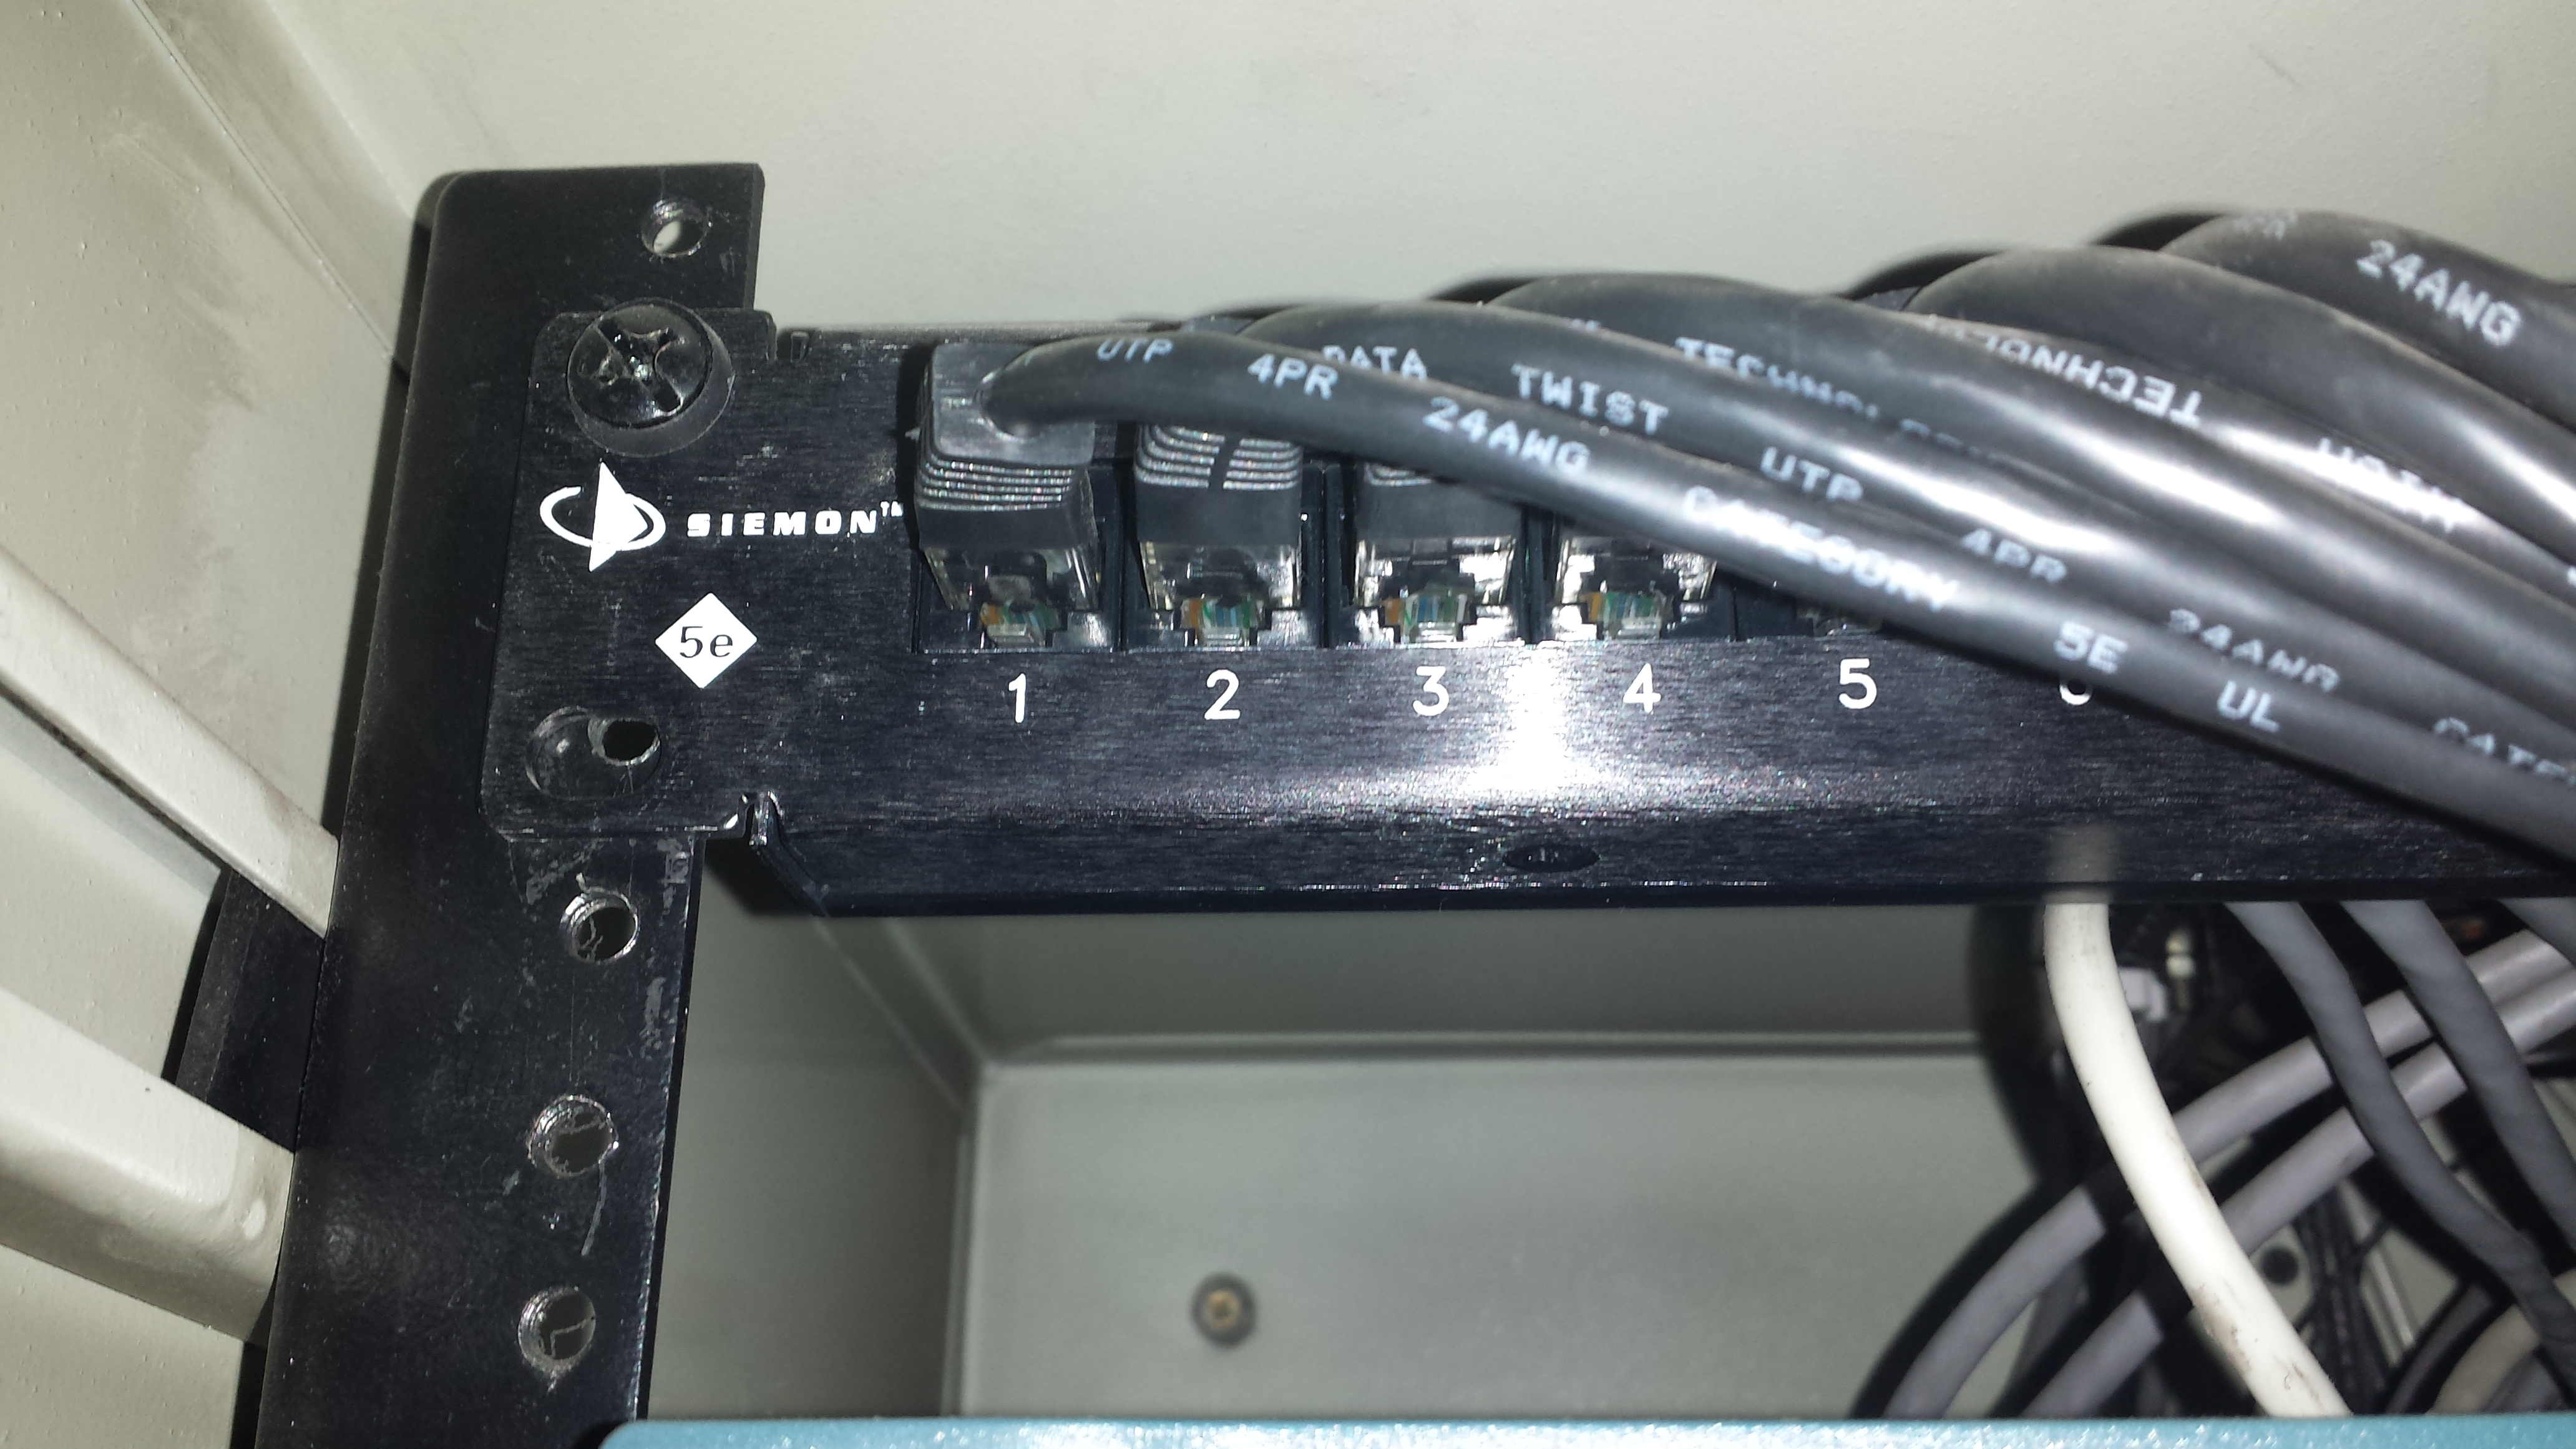
\includegraphics[width=\textwidth]{cablecat5e.jpg}
		\end{figure}
		\item{\bf-Especificaciones:}
		\begin{itemize}
			\item Cubierta y pares sin apantallar.\\
			\item Excede los requerimientos propuestos por la normativa TIA /EIA 568 B .2 ,ISO/IEC 11801 Categoría 5E.\\
			\item Retardante a la llama y cero halógenos según el Standard IEC 60332-3 Cat C.\\
			\item Soporta aplicaciones de hasta 125 MHz de ancho de banda.\\
			\item Codificación de colores para cada uno de los pares\\
			\item Distribuido en cajas de 305 m con bobina interna para facilitar el tendido del cable.\\
			\item Cumple con las normativas de medioambiente CE y RoHS.\\
		\end{itemize}
		\item{\bf-Tipo:} Patch Panel\\
		\item{\bf-Modelo:} Siemon HD5-24 Cat 5e 24 puertos\\
		\begin{figure}[h]
    		\centering
    	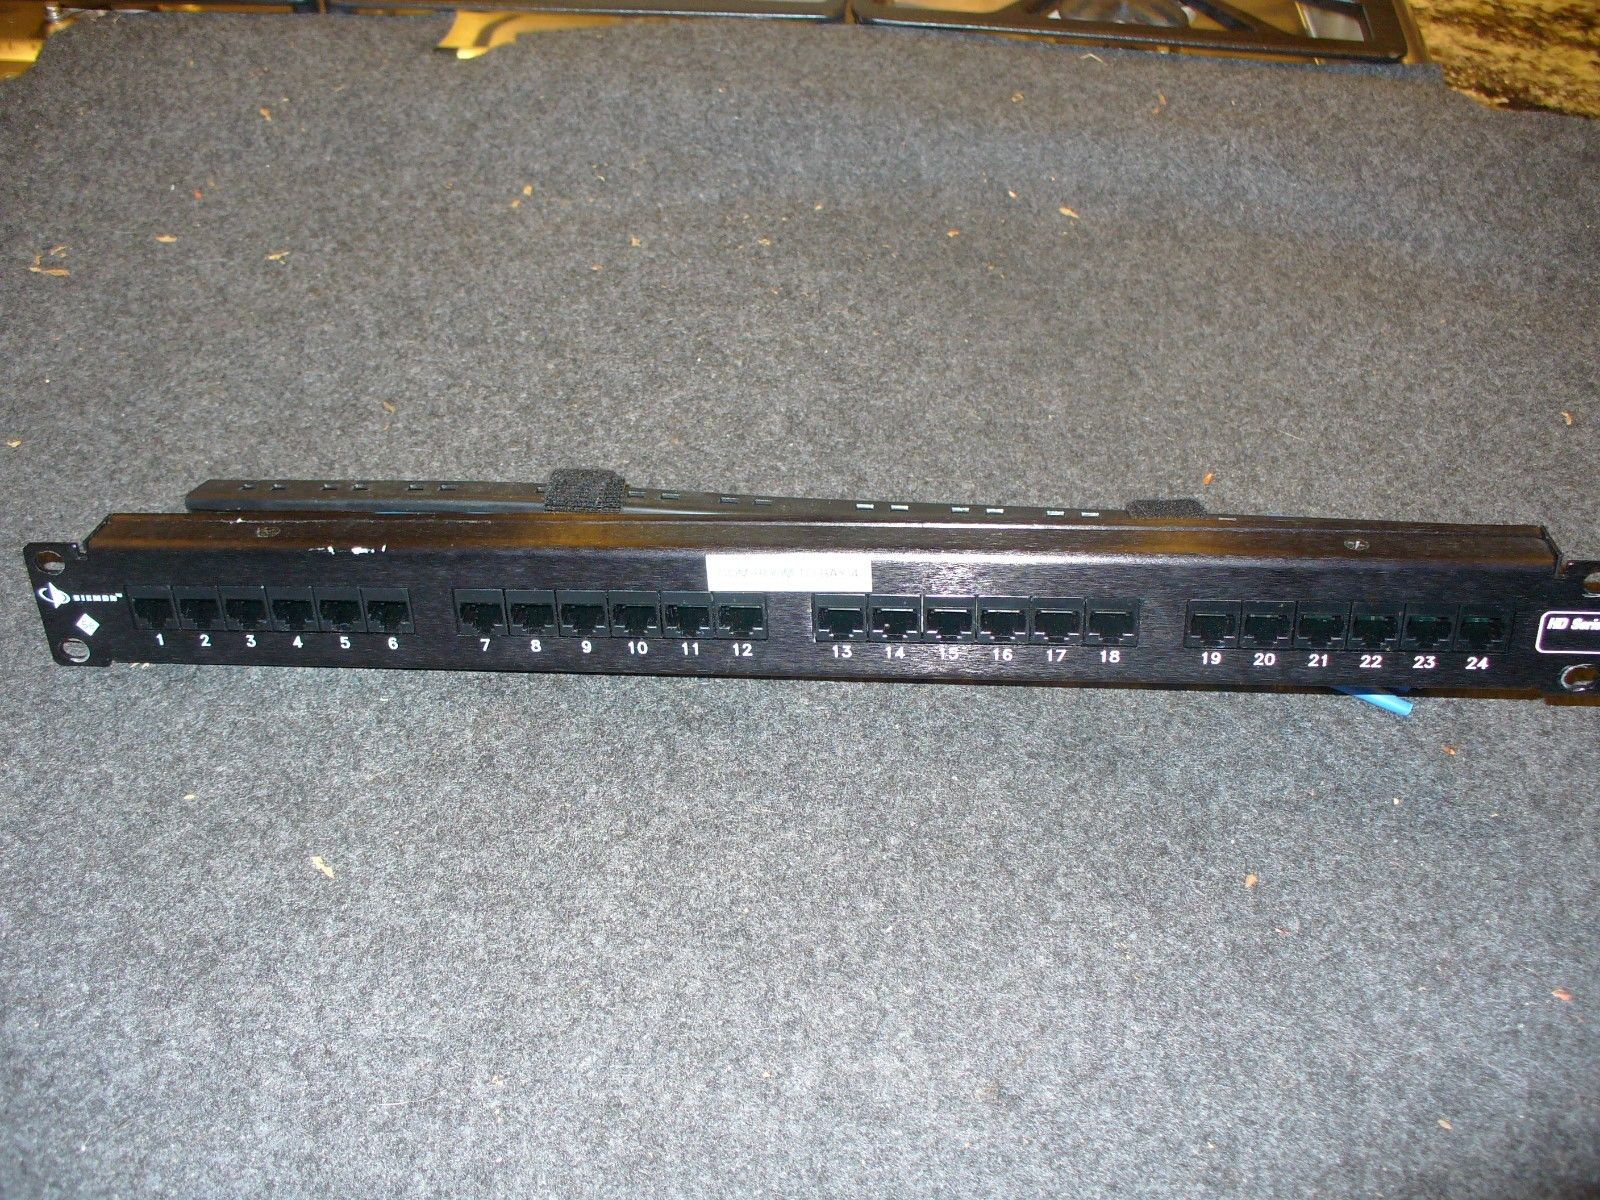
\includegraphics[width=\textwidth]{patchpanel.jpg}
		\end{figure}
		\item{\bf-Especificaciones:}
		\begin{itemize}
			\item Estándares de red: IEEE 802.3, IEEE 802.3ab, IEEE 802.3u\\
			\item Tecnología de cableado: 10/100/1000Base-T(X)\\
			\item Características de red: LAN\\
			\item Color del producto: Negro\\
			\item Materiales: Metal\\
			\item Montaje en rack: 1U\\
		\end{itemize}
	\end{itemize}"
	\section{Información de los dispositivos}
		Para esta actividad abrimos un terminal y ejecutamos el comando "ifconfig" y se desplegó lo siguiente:\\
		\begin{figure}[h]
    		\centering
    	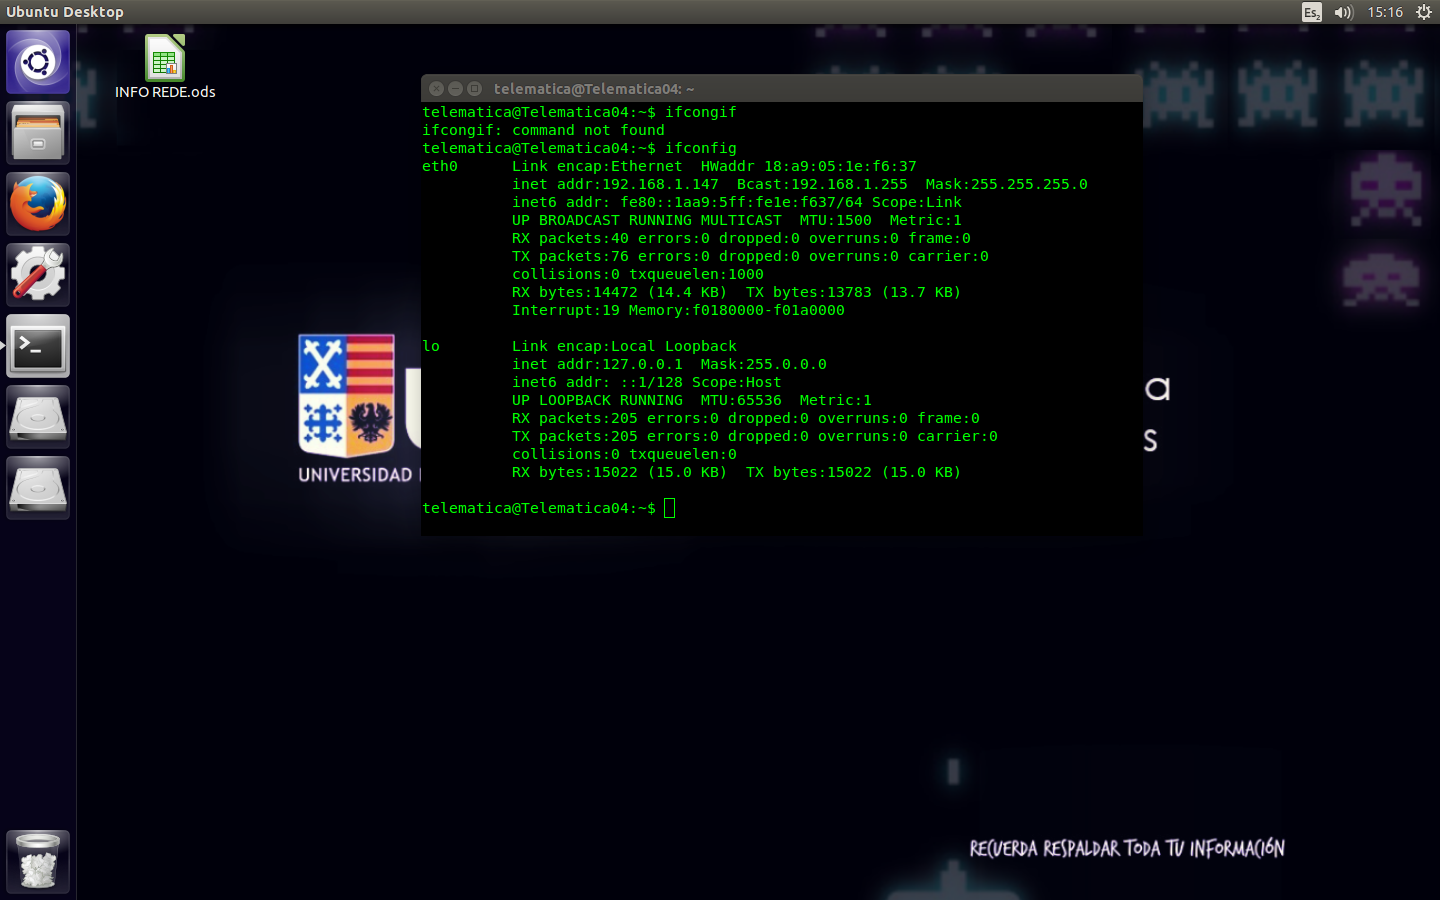
\includegraphics[width=\textwidth]{Terminal.png}
		\end{figure}
		(imagen referencial tomada de otro laboratorio.)\\
		Si observamos la imagen lo que está encerrado en un círculo rojo representa la MAC del equipo y lo encerrado en un
		círculo azul representa la IP del mismo. Al repetir este proceso en cada uno de los computadores de la sala nos    
		dimos cuenta que tanto la MAC como la IP seguían un patrón, en el caso de la MAC los 3 primeros pares de caracteres
		eran iguales en todos los equipos, esto nos dice que las tarjetas de red de todos ellos son del mismo fabricane,      
		el prefijo que se repite es el 40:A8:F0 por lo tanto pudimos llegar a la conclusión de que Hewlett Packard es el      
		fabricante de estas. En el caso de la dirección IP de los computadores solo diferían en los 3 últimos dígitos, ya     
		que al ser una red interna el último número de la dirección debe ser distinto para cada equipo para de esta manera    
		identificar a cada uno.
	\section{Diagrama de red}
		\includegraphics[width=\textwidth]{diagramaf.png}
		Como se observa en el diagrama de red, los computadores están conectados por un cable de red uno por uno 
		con el patch panel, el cual hará que los cables se situen con una mejor distribución física 
		en el espacio.\\
		Gracias a esta descripción se plantea que la topología utilizada en el laboratorio de informática es de tipo estrella 
 		puesto que todos los ordenadores están conectados a un nodo central. Este sistema es muy costoso siendo comparado 
 		junto con las topologias de tipo anillo o tren, ya que para poder conectar cada dispositivo al switch se necesita un
 		cable nuevo de el mismo tamaño, pero al mismo tiempo aporta una caracteristica muy importante la cual es una fácil 
 		detección de problemas y si es que algun cable de red se llegara a romper o a tener problemas solo perderá la conexión
 		ese dispositivo. Aun así si es que el switch se llega a dañar de alguna forma esto afectaría al sistema completo ya
 		que solo depende de éste.
\chapter{Conclusión}
                Gracias a esta experiencia en el laboratorio hemos logrado comprender como funciona un sistema de redes completo 
                incluyendo sus principales componentes, como los cables de red, el patch panel y el switch, la forma en la cual son 
                conectados estos mismos, la utilidad de la dirección IP, la dirección MAC y las topologías que se podrían haber 
                implementado en la configuración de las conexiones. La topología que se está utilizando en el laboratorio de 
                informática es la que según los integrantes del grupo, es la que se adecua a las necesidades existentes, aunque esta 
                requiera de un presupuesto más alto. Además se genera un orden lógico entre los dispositivos de redes al poseer en 
                la sala solamente equipos de un mismo modelo.
\end{document}
